\documentclass[titlepage=true, parskip=full]{scrartcl}
\usepackage[utf8]{inputenc} % use utf8 file encoding for TeX sources
\usepackage[T1]{fontenc}    % avoid garbled Unicode text in pdf
\usepackage{palatino}	      % because "Computer Modern" standard font is illegible
\usepackage{mathpazo}
\usepackage{amsmath}
\usepackage[ngerman]{babel}  % german hyphenation, quotes, etc
\usepackage{hyperref}       % detailed hyperlink/pdf configuration
\hypersetup{                % ‘texdoc hyperref‘ for options
	pdftitle={PSE: Testbericht},%
	bookmarks=true,%
}
\usepackage{graphicx}       % provides commands for including figures
\usepackage{csquotes}       % provides \enquote{} macro for "quotes"
\usepackage[nonumberlist, numberedsection]{glossaries}     % provides glossary commands
\usepackage{enumitem}
\usepackage{tikz}
%\usepackage{tikz-uml}
%\usepackage{tikz-er2}
\usepackage{comment}
\usepackage{array}
\usepackage{longtable}
\usepackage{hhline}
\usepackage{placeins}
\usepackage{needspace}
\usepackage[toc, page]{appendix}
\usepackage{tabularx}
\usepackage{tabulary}
\usepackage{multirow}
\usepackage{multicol}
\usepackage{rotating}
\usepackage{microtype}
\usepackage{MnSymbol}
\usetikzlibrary{positioning}
\usepackage{pgfgantt}
\usepackage{float}
%\usepackage{listings}
\usepackage{xcolor}

\colorlet{punct}{red!60!black}
\definecolor{background}{HTML}{EEEEEE}
\definecolor{delim}{RGB}{20,105,176}
\colorlet{numb}{magenta!60!black}

% Kommandos für Atomare und JSON-Werte:
\newcommand{\jsonatom}[1]{$\langle\textnormal{\textit{#1}}\rangle$}
\newcommand{\jsonobj}[1]{$\llangle\textnormal{\textit{#1}}\rrangle$}
\newcommand{\jsonpart}[2]{$\llangle\textnormal{\textit{#1}\,[#2]}\rrangle$}

\lstdefinelanguage{json}{
    basicstyle=\normalfont\ttfamily,
    numbers=left,
    numberstyle=\scriptsize,
    escapeinside={(*}{*)},
    stepnumber=1,
    numbersep=8pt,
    showstringspaces=false,
    breaklines=true,
    frame=lines,
    backgroundcolor=\color{background},
    literate=
     *{0}{{{\color{numb}0}}}{1}
      {1}{{{\color{numb}1}}}{1}
      {2}{{{\color{numb}2}}}{1}
      {3}{{{\color{numb}3}}}{1}
      {4}{{{\color{numb}4}}}{1}
      {5}{{{\color{numb}5}}}{1}
      {6}{{{\color{numb}6}}}{1}
      {7}{{{\color{numb}7}}}{1}
      {8}{{{\color{numb}8}}}{1}
      {9}{{{\color{numb}9}}}{1}
      {:}{{{\color{punct}{:}}}}{1}
      {,}{{{\color{punct}{,}}}}{1}
      {\{}{{{\color{delim}{\{}}}}{1}
      {\}}{{{\color{delim}{\}}}}}{1}
      {[}{{{\color{delim}{[}}}}{1}
      {]}{{{\color{delim}{]}}}}{1},
}


%\usepackage[vlined]{algorithm2e}
% see http://ctan.math.utah.edu/ctan/tex-archive/macros/latex/contrib/algorithm2e/doc/algorithm2e.pdf  for more information
\DontPrintSemicolon
\SetKwSwitch{Switch}{Case}{Other}{case}{of}{}{else}{}{}
\SetKw{KwAssert}{assert}
\SetKw{KwInvariant}{invariant}
\SetKw{KwStep}{step}
\SetKw{KwDownto}{downto}	
\SetKw{KwArrayOf}{array of }
\SetKw{KwArray}{array }
\SetKw{KwOf}{ of }
\SetKw{KwNot}{ not }
\SetKw{KwIs}{ is }
\SetKw{KwAnd}{ and }
\SetKw{KwOr}{ or }
\SetKw{KwBreak}{break}
\SetKw{KwThrow}{throw}
\SetKw{KwTrue}{true}
\SetKw{KwFalse}{false}
\SetKwBlock{KwFunc}{function}{}
\SetKwBlock{KwProc}{procedure}{}
\newcommand{\Function}[2]{\KwFunc({#1}){#2}}
\newcommand{\Procedure}[2]{\KwProc({#1}){#2}}
\SetKwData{KwList}{List}
\SetKwData{KwSet}{Set}
\newcommand{\KwListOf}{\KwList \KwOf}
\newcommand{\KwSetOf}{\KwSet \KwOf}
\SetKwComment{Comment}{// }{}
\newcommand{\LComment}[1]{\hspace{-2pt}\Comment*[l]{#1}}
\newcommand{\RComment}[1]{$ \qquad $ \Comment*[h]{#1} \\}
\newcommand{\RCommentNoBreak}[1]{$ \qquad $ \Comment*[h]{#1}}
\newcommand{\MyCommentSty}[1]{\emph{\textcolor{gray}{#1}}}
\SetCommentSty{MyCommentSty}
\SetFuncSty{emph}
\definecolor{kwblue}{rgb}{0.3,0.3,1}
\newcommand{\MyKwSty}[1]{\textcolor{kwblue}{\textbf{#1}}}
\SetKwSty{MyKwSty}
\newcommand{\Call}[2]{\FuncSty{#1}(#2)}
\newcommand{\pluseq}{\mathrel{+}=}
\newcommand{\Var}[1]{\textit{#1}}

% needed to define linebreak points without hyphenation (useful for URL wrapping)
\newcommand{\+}{\discretionary{}{}{}}

\renewcommand{\arraystretch}{1.24}  % for proper row spacing in tables

%%%%%%%%%%%%%%%%%%%%%%%%%%%
% longtable multirow page break insanity fix – http://tex.stackexchange.com/a/52101
\makeatletter
\def\@cline#1-#2\@nil{%
	\omit
	\@multicnt#1%
	\advance\@multispan\m@ne
	\ifnum\@multicnt=\@ne\@firstofone{&\omit}\fi
	\@multicnt#2%
	\advance\@multicnt-#1%
	\advance\@multispan\@ne
	\leaders\hrule\@height\arrayrulewidth\hfill
	\cr
	\noalign{\nobreak\vskip-\arrayrulewidth}}
\makeatother
%%%%%%%%%%%%%%%%%%%%%%%%%%%

% For Christ's sake, I'm sick and tired of this f*cking orphan/widow crap!
\widowpenalty=10000
\clubpenalty=10000
% Source: somewhere on tex.stackexchange.com

\renewcommand{\to}{\longrightarrow} % proper math typography
\newcommand{\NN}{\mathbb{N}}
\newcommand{\RR}{\mathbb{R}}
\newcommand{\QQ}{\mathbb{Q}}

\addto\captionsngerman{\let\appendixtocname\appendixname\let\appendixpagename\appendixname}

% fix hyphenation
\hyphenation{Log-out Log-in Ak-tions Ak-tion ge-öff-net liken dis-liken Like Dis-like No-ti-fi-ca-tion Mo-dule inkl Au-tho-ri-za-tion Web-App Ar-chi-tek-tur-en Ge-ne-rie-rungs Stu-di-en-plan Client außer-dem}

\usepackage{enumitem}
\setlist[itemize]{nosep}
\shorthandon{"}
%\makeglossaries
%%
% % Automatisch generiertes Glossar
%
%\glsaddall % das sorgt dafür, dass alles Glossareinträge gedruckt werden, nicht nur die verwendeten. Das sollte nicht nötig sein!
%
% % Glossareinträge
%
\newglossaryentry{Rest}
{
	name=REST,
	description={Abk. für Representational State Transfer, Programmierparadigma für \glspl{Webservice} auf Basis des HTTP-Protokolls}
}

\newglossaryentry{ECTS-Punkte}
{
	name=ECTS-Punkte,
	description={Leistungspunkte, die für ein erfolgreich absolviertes \gls{Modul} von der Hochschule auf Basis des ECTS-Punktesystems vergibt werden, und mit denen der Arbeitsaufwand gemessen wird},
}

\newglossaryentry{Generierungs-Tool}
{
	name=Generierungs-Tool,
	description={Tool, für die automatische Erstellung bzw. Vervollständigung von Studienpläne},
}


\newglossaryentry{Webservice}
{
	name=Webservice,
	plural=Webservices,
	description={Softwareanwendung, die über ein Netzwerk bereitgestellt wird}
}

\newglossaryentry{Plug-In-Paket}
{
	name=Plug-In-Paket,
	plural=Plug-In-Pakete,
	description={Paket bestehend aus mehreren \glspl{Plug-In}}
}

\newglossaryentry{iMage}
{
	name={iMage},
	description={Bildbearbeitungssoftware der Firma SWT. Bietet im Basispaket nur Funktionalitäten zur Skalierung und Drehung von Bildern}
}

\newglossaryentry{Internetbrowser}
{
	name={Internetbrowser},
	description={Programm, mit dem Websites gefunden, gelesen und verwaltet werden können, mit aktiviertem JavaScript}
}

\newglossaryentry{Online-Shop}
{
	name={Online-Shop},
	description={Internetseite, die Produkte zum Kauf anbietet}
}

\newglossaryentry{KIT}
{
	name=KIT,
	description={Das Karlsruher Institut für Technologie ist die Forschungsuniversität in der Helmholtz-Gemeinschaft. Standort der Universität ist Karlsruhe. }
}

\newglossaryentry{SCC}
{
	name=SCC,
	plural=SCC,
	description={Das Steinbuch Center for Computing ist ein Institut und das zentrale Rechenzentrum des \gls{KIT}s.}
}

\newglossaryentry{Benutzer}
{
	name=Benutzer,
	plural=Benutzer,
	description={Ein am \gls{KIT} eingeschriebener Student, der über ein gültigen Account beim \gls{SCC} verfügt.}
}

\newglossaryentry{Wizard}
{
	name=Wizard,
	plural=Wizards,
	description={Ein Wizard ist ein Subsystem, welches einen \gls{Benutzer} visuell durch eine Systemfunktionalität führt und dabei vom \gls{Benutzer} bestimmte Interaktionen mit dem System fordert.}
}

\newglossaryentry{Drag-and-Drop}
{
	name=Drag-and-Drop,
	description={(deutsch: "Ziehen und Ablegen") Eine Methode zur Bedienung grafischer Benutzeroberflächen bei der grafische Elemente mittels eines Mauszeigers bewegt werden.}
}

\newglossaryentry{Shibboleth Identity Provider}
{
	name=Shibboleth Identity Provider,
	description={Ein genau spezifiziertes System zum Login mittels einer von einer dritten Instanz bereitgestellten Identität.}
}

\newglossaryentry{Studiengang}
{
	name=Studiengang,
	description={Ein vom KIT angebotener, auf einer Studien- und Prüfungsordnung und einem Modulhandbuch basierender Studiengang.}
}

\newglossaryentry{Semester des Studienbeginns}
{
	name=Semester des Studienbeginns,
	description={Das Semester in welchem der \gls{Benutzer} im ersten Fachsemester des \gls{Studiengang}s war.}
}

\newglossaryentry{Modul}
{
	name=Modul,
	plural=Module,
	description={Ein Modul ist ein Teilblock des Studiums, welcher aus verschiedenartigen Veranstaltungen (genannt \glspl{Teilmodul}) bestehen kann und für welchen man nach Ablegung eventueller \glspl{Modulpruefung} eine festgelegte Anzahl an ECTS-Punkten erhält.}
}
\newglossaryentry{Teilmodul}
{
	name=Teilmodul,
	plural=Teilmodule,
	description={Ein Teilmodul ist eine universitäre Veranstaltung, welche als Teil eines Moduls besucht werden kann und mittels einer (wie auch immer gearteten) \gls{Modulpruefung} bestanden werden kann.}
}
\newglossaryentry{Modulpruefung}
{
	name=Modulprüfung,
	plural=Modulprüfungen,
	description={Eine Modulprüfung ist eine Prüfung, welche abgelegt werden muss um ein Modul \glslink{Modul abgeschlossen}{abzuschließen}.}
}
\newglossaryentry{Zur Pruefung angetreten}
{
	name=Zur Pruefung angetreten,
	description={Ein \gls{Benutzer} ist zu einer \gls{Modulpruefung} angetreten, wenn er sich fristgerecht für selbige angemeldet und nicht fristgerecht abgemeldet hat.}
}

\newglossaryentry{Modul abgeschlossen}
{
	name=Modul abgeschlossen,
	description={Ein \gls{Modul} gilt als abgeschlossen, wenn der \gls{Benutzer} alle nach Modulhandbuch notwendigen \glspl{Modulpruefung} bestanden hat.}
}

\newglossaryentry{Modul begonnen}
{
	name=Modul begonnen,
	description={Ein \gls{Modul} gilt als begonnen, wenn der \gls{Benutzer} zu mindestens einer \gls{Modulpruefung} \glslink{Zur Pruefung angetreten}{angetreten} ist.}
}

\newglossaryentry{Studienplan}
{
	name=Studienplan,
	plural=Studienpläne,
	description={Eine Zusammenstellung von Modulen, in welcher enthalten ist wann welches Modul planmäßig \glslink{Modul begonnen}{begonnen} werden soll.}
}
\shorthandoff{"}

\begin{document}
	
\begin{titlepage}
	\centering
	{\huge \bfseries \sffamily Studienplanung als Generierung von Workflows mit Compliance-Anforderungen: Planerstellung und Visualisierung\par}
	\vspace{1cm}
	{\LARGE Testbericht\par}
	\vfill
	\begin{tabular}{>{\Large}c}
		Nada Chatti\\
		\textbf{Daniel Jungkind}\\
		Hannes Kuchelmeister\\
		Ulrike Rheinheimer\\
		Paul Samuel M. Teuber\\
		Tim Niklas Uhl
	\end{tabular}
	\vfill
	15. März 2017
\end{titlepage}
\tableofcontents
\pagebreak

%
% % Hier beginnt die Gliederung des Pflichtenhefts
\section{Einleitung}
Der Implementierungsbericht des Projekts „Studienplanung als Generierung von Workflows mit Compliance-Anforderungen: Planerstellung und Visualisierung“ beschreibt die Umsetzung des zuvor im Pflichtenheft und Entwurf spezifizierten Projekts. In über ????? Zeilen Java-, Javascript-, HTML- und CSS-Code liegt jetzt eine fertige, nur noch zu optimierende Anwendung vor. In diesem Bericht möchten wir dabei auf implementierte und ausgelassen Features eingehen, Änderungen beschreiben und begründen, und die Implementierungsphase (einschließlich aller durchgemachten Nächte) reflektieren.
Zusammenfassend ist dieser Bericht Ende einer arbeitsintensiven, aber erfolreichen Phase, die als Endprojekt ein einmalig sinnvolles, dringendnotweniges und jedem Studenten zu empfehlendes Studienplanungshilfsmittel zur Verfügung stellt.




\FloatBarrier
\section{Testfälle}

Es wurden weitere Unit- und Integrationstests hinzugefügt, mit welchen zusätzliche Produkt-Stabilität einhergeht. Hier erfolgt nun eine Auflistung aller Unit- und Integrationstests.

\FloatBarrier
\subsection{Server}

\subsubsection*{Unit-Tests}

\begin{longtable}{| >{\hspace{0pt}} p{.26\textwidth} | >{\hspace{0pt}} p{.45\textwidth} | >{\hspace{0pt}} p{.19\textwidth} |}
	\hline
	\textbf{Testklasse} & \textbf{Beschreibung} & \textbf{Status} \\ 
	\hhline{|=|=|=|}  
	\endfirsthead
	\endhead
	CategoryTest & Getter und Setter für \texttt{Category} getestet & ERFOLGREICH \\
	\hline
	DisciplineTest & Getter und Setter für \texttt{Discipline} getestet & ERFOLGREICH \\
	\hline
	SemesterTest & Test der Semester-Abstandsberechnung zwischen:
	\begin{itemize}
		\item zwei Wintersemestern
		\item zwei Sommersemestern
		\item zwischen Winter- und Sommersemester
		\item zwischen Sommer- und Wintersemester
	\end{itemize}
	Test der compareTo-Methoden \\
	Test der plus-Methode & ERFOLGREICH \\
	\hline
	StandardVerifierTest & Testet, ob der \texttt{StandardVerifier} folgendes erkennt:
	\begin{itemize}
		\item fehlende Pflichtmodule
		\item Verletzung von Rule-Group"=Bedingungen
		\item Verletzung von Bereichsbedingungen (Fields)
	\end{itemize} & ERFOLGREICH \\
	\hline
	StandardVerifierConstraintTest & Testet ob der die Verletzung folgender \texttt{ConstraintTypes} in unterschiedlichen Ausartungen erkennt:
	\begin{itemize}
		\item Verletzung von Überlappung 
		\item Verletzung von Plan"=Zusammengehörigkeit 
		\item Verletzung von Semester"=Zusammengehörigkeit 
		\item Verletzung von Voraussetzungen
	\end{itemize}
	Dadurch wurden auch die \texttt{isValid}-Methoden der entsprechenden \texttt{ConstraintTypes} getestet & ERFOLGREICH \\
	\hline
	SimpleGeneratorTest & Testet die \texttt{generate}-Methode des \texttt{SimpleGenerator}.
	Ein Plan mit einem einzelnen \texttt{ModuleEntry} wird:
	\begin{itemize}
		\item anhand der Benutzer"=Präferenzen und \texttt{Constraint}s verschiedener Art vervollständigt und modifiziert
		\item anhand einer Zielfunktion optimiert
	\end{itemize}
	Dafür werden sog. Mock-Objekte benutzt, die nur zum Testen erstellt wurden, d.h. bei der echten Verwendung des Systems werden diese nicht benutzt werden, sondern stattdessen die Daten aus der Datenbank. Das Verhalten von Methoden der Klassen \texttt{ModuleDao} und \texttt{Plan} wurde hierfür mittels Mockito angepasst. & ERFOLGREICH\\
	\hline
	NodesListTest & Testet die topologische Sortierung der Klasse \texttt{NodesList}. & ERFOLGREICH\\
	\hline
	VerificationManager & Getter für \texttt{Verifier} getestet. & ERFOLGREICH\\
	\hline
	ConditionTest & Factory-Methoden getestet & ERFOLGREICH \\
	\hline
	ContainsFilterDescriptorTest, ListFilterDescriptorTest, RangeFilterDescriptorTest, FilterDescriptorTest,  & Korrekte JSON-Serialisierung, Parsen der Filterdaten aus einem Request getestet; dabei auch ungültige Eingaben überprüft & ERFOLGREICH \\
	\hline
	FilterDescriptorProviderTest & Invarianten des Providers getestet (untersch. URI"=Identifier u. IDs, jeder veröffentlichte Filter kann mit dem Identifier gefunden werden) & ERFOLGREICH \\
	\hline
	MultiFilterTest & Korrekte Listenglättung der Sub-Condition-Listen getestet & ERFOLGREICH \\
	\hline
	TrueFilterTest & Rückgabe einer leeren Condition-Liste getestet & ERFOLGREICH \\
	\hhline{|=|=|=|}  
\end{longtable}

\subsubsection*{Integrations-Tests}

\begin{longtable}{| >{\hspace{0pt}} p{.26\textwidth} | >{\hspace{0pt}} p{.45\textwidth} | >{\hspace{0pt}} p{.19\textwidth} |}
	\hline
	\textbf{Testklasse} & \textbf{Beschreibung} & \textbf{Status} \\ 
	\hhline{|=|=|=|}  
	\endfirsthead
	\endhead
	DisciplinesResourceIntegrationTest & Überprüft die korrekte JSON-Serialisierung von GET /disciplines. & ERFOLGREICH \\
	\hline
	FieldsResourceIntegrationTest & Überprüft die korrekte JSON-Serialisierung von GET /fields. & ERFOLGREICH \\
	\hline
	ObjectiveFunctionResourceIntegrationTest & Überprüft die korrekte JSON-Serialisierung von GET /objective-functions. & ERFOLGREICH \\
	\hline
	FilterResourceIntegrationTest & Überprüft die korrekte JSON-Serialisierung von GET /filters (die drei Typen range, list und contains samt zugehöriger Spezifikation). & ERFOLGREICH \\
	\hline
	StudentResourceIntegrationTest & Überprüft, ob der Nutzer beim Neuanlegen korrekt initialisiert ist; das Setzen von Fachrichtung und Studienstart funktioniert; fehlerhafte Fachrichtungen/Studienstarts (zukünftig/prähistorisch) abgefangen werden; bestandene Module korrekt gesetzt werden; fehlerhafte bestandene Module (falsches Modul, falsches Semester) abgefangen werden; die JSON-Rückgaben korrekt serialisiert werden und eine Autorisierung vor dem Zugriff auf die Ressourcen verlangt wird. & ERFOLGREICH \\
	\hline
	ModuleResourceIntegrationTest & Überprüft, ob GET /modules/id korrekt als JSON serialisiert wird und auch die korrekten Daten gesendet werden; testet mehrere Filteraufrufe auf korrekte Rückgabe sowie fehlerhafte Eingabe. & ERFOLGREICH \\
	\hline
	
	PlansResourcePlanCreationIntegrationTest & 
		folgendes wurde überprüft:
		\begin{itemize}
			\item Anlegen eines Plans möglich
			\item korrekte Serialisierung aller Pläne eines Nutzers
			\item doppelte Plannamen werden abgefangen
			\item ungültige Plannamen werden abgefangen (leerer Name, zu langer Name)
			\item Zugriff nur autorisiert möglich
		\end{itemize}
		& ERFOLGREICH \\ \hline
	PlansResourcePlanEditIntegrationTest & 
	folgendes wurde überprüft:
	\begin{itemize}
		\item Planumbenennung möglich; doppelte Namen, leere Namen, zu lange Namen werden abgefangen
		\item korrekte Serialisierung eines Plans
		\item Platzierung von Modulen im Studienplan
		\item Bewegung von Modulen im Studienplan
		\item Entfernen von Modulen aus dem Studienplan
		\item Setzen und Entfernen von Modulpräferenzen
		\item Zugriff auf die Exportfunktion
		\item Zugriff auf Ressourcen nur autorisiert möglich
	\end{itemize}
	Dies beinhalten auch das Überprüfen ungültiger Eingabeparameter.
	& ERFOLGREICH \\
	
	\hhline{|=|=|=|}  
\end{longtable}

\FloatBarrier
\subsection{Client}
\subsubsection*{Unit-Tests}
\begin{longtable}{| >{\hspace{0pt}} p{.2\textwidth} | >{\hspace{0pt}} p{.45\textwidth} | >{\hspace{0pt}} p{.25\textwidth} |}
	\hline
	\textbf{Testfall} & \textbf{Beschreibung} & \textbf{Status} \\ 
	\hhline{|=|=|=|}  
	\endfirsthead
	\endhead
	
	%===============================================================================================
	ModuleCollection"=Initialisierung & Wird eine ModuleCollection für gegebene Daten erfolgreich initialisiert?  & ERFOLGREICH \\ \hline
	ModuleConstraint"=Initialisierung & Wird ein ModuleConstraint für gegebene Daten erfolgreich initialisiert? & ERFOLGREICH \\ \hline
	Module"=Initialisierung & Wird ein Modul für gegebene Daten erfolgreich initialisiert? & ERFOLGREICH \\ \hline
	Preference"=Initialisierung & Wird eine Preference für gegebene Daten erfolgreich initialisiert? & ERFOLGREICH \\ \hline
	Plan"=Initialisierung & Wird ein Plan für gegebene Daten erfolgreich initialisiert? & ERFOLGREICH \\ \hline
	Discipline"=Initialisierung & Wird eine Discipline für gegebene Daten erfolgreich initialisiert? & ERFOLGREICH \\ \hline
	Filter"=Initialisierung & Wird ein Filter für gegebene Daten erfolgreich initialisiert? & ERFOLGREICH \\ \hline
	LanguageManager"=Funktion & Gibt der Language Manager die richtigen Textbausteine zurück? & ERFOLGREICH \\ \hline
	NotificationCollection"=Initialisierung & Gibt getInstance() das richtige Objekt zurück? & ERFOLGREICH \\ \hline
	ObjectiveFunctionCollection"=Initialisierung & Wird eine ObjectiveFunctionCollection für gegebene Daten erfolgreich initialisiert? & ERFOLGREICH \\ \hline
	TemplateManager"=Funktion & Gibt der TemplateManager die richtige HTML"=Ausgabe zurück? & ERFOLGREICH \\ \hline
	CookieSync"=Funktion & Speichert/Lädt CookieSync ein Modell erfolgreich? & ERFOLGREICH \\ \hline
	OAuthSync"=Funktion & Übergibt OAuthSync beim Speichern/Laden die richtigen Header? & ERFOLGREICH \\ \hline
	MainView"=Funktion & Lädt die MainView die richtigen Views und zeigt diese an? & ERFOLGREICH \\	 
	\hhline{|=|=|=|}   
\end{longtable}

\subsubsection*{Integrations-Tests}
\begin{longtable}{| >{\hspace{0pt}} p{.2\textwidth} | >{\hspace{0pt}} p{.45\textwidth} | >{\hspace{0pt}} p{.25\textwidth} |}
	\hline
	\textbf{Testfall} & \textbf{Beschreibung} & \textbf{Status} \\ 
	\hhline{|=|=|=|}  
	\endfirsthead
	\endhead
	
	%===============================================================================================
	DisciplineCollection & Test der Kommunikation zwischen DisciplineCollection und Server-Mock /disciplines & ERFOLGREICH \\ \hline
	FieldCollection & Test der Kommunikation zwischen FieldCollection und Server-Mock /fields & ERFOLGREICH \\ \hline
	FilterCollection & Test der Kommunikation zwischen FilterCollection und Server-Mock /filters & ERFOLGREICH \\ \hline
	Module & Test der Kommunikation zwischen Module und Server-Mock /plans/\{id\}/modules/\{id\} & ERFOLGREICH \\ \hline
	ModuleCollection & Test der Kommunikation zwischen ModuleCollection und Server-Mock /plans/\{id\}/modules & ERFOLGREICH \\ \hline
	ObjectiveFunctionCollection & Test der Kommunikation zwischen ObjectiveFunctionCollection und Server-Mock /objective-functions  & ERFOLGREICH \\ \hline
	Plan & Test der Kommunikation zwischen Plan und Server-Mock /plans/\{id\} & ERFOLGREICH \\ \hline
	PlanCollection & Test der Kommunikation zwischen PlanCollection und Server-Mock /plans & ERFOLGREICH \\ \hline
	ProposedPlan & Test der Kommunikation zwischen ProposedPlan und Server-Mock /plans/\{id\}/proposal/\{objective-function\} & ERFOLGREICH \\ \hline
	Student & Test der Kommunikation zwischen Student und Server-Mock /student & ERFOLGREICH \\ \hline
	
\end{longtable}

\FloatBarrier
\subsection{Server-Coverage-Daten}

Im Folgenden sind Coverage-Statistiken zur Server-Überdeckung aufgeführt. 

\paragraph{Unit-Tests} Für das rest-Package wurden keine Unit-Tests verfasst, weshalb es hier auch nicht aufgeführt ist; die REST-Schnittstellen werden sinnvollerweise in den Integrationstests abgedeckt. Da der Plugin-Manager weitestgehend kastriert wurde, erschien eine größere Abdeckung nicht mehr nötig; genauso auch wie bei vielen primitiven Gettern und Settern im Model.

\begin{longtable}{| >{\hspace{0pt}} p{.26\textwidth} | >{\hspace{0pt}} p{.45\textwidth} | }
	\hline
	\textbf{Package} & \textbf{Zeilenüberdeckung} \\ 
	\hhline{|=|=|}  
	\endfirsthead
	\endhead
	%%
	filter & 81 \% \\
	\hline
	generation & 71 \% \\
	\hline
	model & 36 \% \\
	\hline
	pluginmanager & 14 \% \\
	\hline
	verification & 85 \% \\
	\hhline{|=|=|} 
	\textbf{Gesamt} & \textbf{57 \%} \\
	\hhline{|=|=|} 
	\caption{Unit-Test-Überdeckung Server}
\end{longtable}

\paragraph{Integrations-Tests} Aufgrund von Schwierigkeiten beim Zusammenspiel von JaCoCo und unserer Tomcat"=Serverumgebung sind für Integrationstests keine Coverage-Daten verfügbar. Als groben Überblick diene stattdessen die manuell bestimmte Methodenüberdeckung für die einzelnen REST"=Ressourcen. Auf Integrationstests für Verifzierung und Generierung wurde verzichtet, da diese schon ausreichend mit Unit-Tests abgedeckt sind.

\begin{longtable}{| >{\hspace{0pt}} p{.26\textwidth} | >{\hspace{0pt}} p{.45\textwidth} | }
	\hline
	\textbf{REST-Ressource} & \textbf{Methodenüberdeckung} \\ 
	\hhline{|=|=|}  
	\endfirsthead
	\endhead
	%%
	/disciplines & 100 \% \\
	\hline
	/fields & 100 \% \\
	\hline
	/filters & 100 \% \\
	\hline
	/modules & 100 \% \\
	\hline
	/objective-functions & 100 \% \\
	\hline
	/plans & 72 \% \\
	\hline
	/student & 100 \% \\
	\hhline{|=|=|} 
	\textbf{Gesamt} & \textbf{ 96 \%} \\
	\hhline{|=|=|} 
	\caption{Integrations-Test-Überdeckung Server}
\end{longtable}

\FloatBarrier
\subsection{Client-Coverage-Daten}
Die beim Client gemessene Testüberdeckung beträgt 44,98\%. Leider ist dieser Wert aus mehreren Gründen ungenau.
\paragraph{Testen der Nutzeroberfläche}
Neben den vorhandenen Unit- und Integrations-Tests, welche von dieser Metrik erfasst werden, wurden auch eine Vielzahl von manuellen und halb-automatisierten Nutzeroberflächen-Tests durchgeführt (teilweise manuell, teilweise mit Hilfe der Selenium-IDE). Diese Testfälle orientierten sich insbesondere an den im Pflichtenheft festgelegten globalen Testfällen. Aus technischen Gründen können diese Tests jedoch nicht in die Testüberdeckung miteingerechnet werden.\\
Dennoch waren insbesondere diese Tests sehr effektiv beim Aufdecken von Fehlern, da durch das Bedienen der Nutzeroberfläche die Kommunikation und das Zusammenspiel der verschiedenen Subsysteme exzellent überprüft werden konnte. Die hier genannten Testmethoden haben uns dabei geholfen, viele Fehler in der Software zu finden und zu beseitigen.
\paragraph{Daten im Code}
Aus Performance-Gründen hatten wir uns bereits in der Entwurfsphase dafür entschieden, verschiedene Daten wie Templates und Sprachdaten zur Compilezeit in den Code miteinzubauen. Hierdurch wurden die notwendigen Serveranfragen beim Ausführen des Clients im Webbrowser deutlich reduziert. Dies wirkt sich sehr positiv auf die Geschwindigkeit der Anwendung aus, da zur Laufzeit lediglich die Daten der REST-Schnittstelle geladen werden müssen. Gleichzeitig führt diese Entscheidung allerdings zu Ungenauigkeiten bei der Messung der Testüberdeckung, da diese Daten ebenfalls als \enquote{Codezeilen} aufgefasst werden.

\FloatBarrier
\section{Änderungen an Testszenarien aus dem Pflichtenheft}

\FloatBarrier
\subsection{Geänderte Anwendungsfälle}

Durch die während der Entwicklung geänderten Anforderungen erfordern manche Anwendungsfälle zusätzliche Anpassungen, welche hier aufgelistet sind. Gestrichen wurden Anwendungsfälle, deren zugrundeliegende Produktfunktionalität entfernt wurde.

\begin{longtable}{| >{\hspace{0pt}} p{.32\textwidth} | >{\hspace{0pt}} p{.63\textwidth} |}
	\hline
	\textbf{Anwendungsfall} & \textbf{Änderung} \\ 
	\hhline{|=|=|}  
	\endfirsthead
	\endhead
	%%
	A10: Erstanmeldung / \newline A20: Login 
	& Auf Einbindung des Shibboleth Identity Providers wurde (wie angekündigt) verzichtet. \\
	\hline
	A40: Profil bearbeiten
	& Eingabe von Studienbeginn/Studiengang nur bei Erstanmeldung möglich; „Konto speichern“ kehrt nicht zur letzten offenen Seite zurück. Der Nutzer kann außerdem sein Konto löschen. \\
	\hline
	A50: Neuen Studienplan anlegen
	& Das Namens-Popup hat keine Voreinstellung. \\
	\hline
	A70: Studienplan duplizieren
	& Es wird nach einem neuen Namen für den Plan gefragt. (Benutzerfreundlicher) \\
	\hline
	A85: Studienplan exportieren
	& Es wird eine HTML-Zusammenfassung des Studienplans im Browser angezeigt. \\
	\hline
	A90: Mehrere Studienpläne löschen
	& Duplizieren und Teilen wurden entfernt und das Aktions"=Wahlfeld durch eine einzige Schaltfläche ersetzt. \\ 
	\hline
	A100: Studienpläne vergleichen
	& Entfernt. \\
	\hline
	A110: Module filtern
	& Filtern nach Fachrichtung und Vorkommen im Plan entfernt; Filtern nach Bereich hinzugefügt. \\
	\hline
	A130: Modulinfo-Leiste
	& Möglichkeit zur Bewertung entfernt; Modul"=Constraints werden nun angezeigt. \\
	\hline
	A140: Modul einfügen
	& Module können auch in abgeschlossene Semester eingefügt werden. \\
	\hline
	A170: Änderung rückgängig machen
	& Entfernt. \\
	\hline
	A210: Semesterzeile löschen
	& Da Zeilen nicht explizit gespeichert werden und leere Zeilen gar nicht: Entfernt. \\
	\hline
	A215: Abgeschlossene Semester ein-/ausblenden
	& Entfernt. \\
	\hline
	A220: Studienplan überprüfen
	& Es gibt keine Tooltips beim Drüberfahren mit der Maus, stattdessen werden die Verifizierungsergebnisse gesammelt als Popup angezeigt. \\
	\hhline{|=|=|}
\end{longtable}

\subsubsection*{Testergebnisse}

\begin{longtable}{| >{\hspace{0pt}} p{.73\textwidth} | >{\hspace{0pt}} p{.20\textwidth} |}
	\hline
	\textbf{Anwendungsfall} & \textbf{Status} \\ 
	\hhline{|=|=|}  
	\endfirsthead
	\endhead
	%%
	A10: Erstanmeldung & ERFOLGREICH \\
	\hline
	A20: Login & ERFOLGREICH \\
	\hline
	A30: Logout & ERFOLGREICH \\
	\hline
	A40: Profil bearbeiten & ERFOLGREICH \\
	\hline
	A50: Neuen Studienplan anlegen & ERFOLGREICH \\
	\hline
	A55: Studienplan anzeigen / A57: schließen & ERFOLGREICH \\
	\hline
	A60: Plan umbenennen & ERFOLGREICH \\
	\hline
	A70: Plan duplizieren & ERFOLGREICH \\
	\hline
	A80: Plan löschen & ERFOLGREICH \\
	\hline
	A85: Plan exportieren & ERFOLGREICH  \\
	\hline
	A90: Mehrere Studienpläne löschen & ERFOLGREICH \\
	\hline
	A110: Module filtern & ERFOLGREICH  \\
	\hline
	A130: Modulinfo anzeigen & ERFOLGREICH  \\
	\hline
	A140: Modul einfügen & ERFOLGREICH  \\
	\hline
	A150: Modul löschen & ERFOLGREICH  \\
	\hline
	A160: Modul verschieben & ERFOLGREICH  \\
	\hline
	A180/190: Modul positiv/negativ bewerten & ERFOLGREICH  \\
	\hline
	A200: Semesterzeile einfügen & ERFOLGREICH  \\
	\hline
	A220: Plan überprüfen & ERFOLGREICH \\
	\hline
	A230: Plan vervollständigen & ERFOLGREICH \\
	\hhline{|=|=|}
\end{longtable}



\FloatBarrier
\subsection{Geänderte Testszenarien}

Im Folgenden eine Auflistung der Testszenarien, deren Änderungen aus den angepassten Anwendungsfällen hervorgehen.



\FloatBarrier
\section{Geänderte Produktfunktionen}

Es folgt eine Auflistung der hinzugefügten, geänderten und entfernten Produktfunktionen.

Hinzugefügt:
\begin{itemize}
	\item Bereichs-Filter in der Suchleiste
	\item Hilfe-Funktion: Bietet dem User Hilfestellung zur Bedienung und erläutert die Funktionen.
\end{itemize}

\FloatBarrier
\section{Behobene Fehler}

Es folgt eine Auflistung aller behobenen Produktmängel. (Bei mit „---“ markierten Spalten erschien die Nennung von Ursache/Behebung überflüssig.)

% Etwa 70 Mängel.

\begin{longtable}{| >{\hspace{0pt}} p{.32\textwidth} | >{\hspace{0pt}} p{.32\textwidth} | >{\hspace{0pt}} p{.32\textwidth} | }
	\hline
	\textbf{Fehler} & \textbf{Ursache}  & \textbf{Behebung} \\ 
	\hhline{|=|=|=|}
	\endfirsthead
	\endhead
	%%
	expires\_in-Daten werden nicht in SessionInformation gespeichert/verarbeitet & --- & --- \\
	\hline
	Modulinfo-Leiste zeigt nichts an und lässt sich nicht schließen. & Schließen: Ein Event war nicht richtig registriert; Keine Anzeige: Falsche Übergabe der Daten an Template & --- \\
	\hline
	Module können in jedem beliebigen Turnus abgelegt werden & Client/Server validieren die Eingabe nicht & Validierung ob das gewählte Semester mit dem Modul-Turnus kompatibel ist \\
	\hline
	Nutzer wird nach Löschen des Kontos nicht ausgeloggt & Fehlende/Fehlerhafte URI-Weiterleitung & --- \\
	\hline
	Beim Erstlogin kann ein Semester aus der Zukunft erstellt werden & Fehler beim dynamischen Erstellen der Auswahlmöglichkeiten auf Basis des aktuellen Datums & Erstlogin-Wizard zeigt keine Semester aus der Zukunft mehr an \\
	\hline
	Modulsuchleisten"=Scrollbar wird nach Filter-Anwendung zurückgesetzt & Der Lade-Bildschirm führte automatisch zu einem neu-rendern der Seite & --- \\
	\hline
	Server akzeptiert Modulbelegungen in nicht-positive Semester & Fehlende Validierung der Eingabe & Eingabevalidierung ergänzt \\
	\hline
	Der Kategorie-Filter kann nicht verändert werden & Bei Neu-Rendern des Felds wurde das aktuell ausgewählte Feld nicht berücksichtigt & Aktuell ausgewähltes Feld bei Rendering als ausgewählt setzen \\
	\hline
	Bestandene Module erscheinen nach Verifizierung fehlerhaft, sollten aber ignoriert werden & \texttt{SemesterLinkConstraint\#isValid()} berücksichtigte abgeschlossene Module nicht & Wenn beide Module im Plan vorhanden und mind. eines von beiden bestanden ist, wird \texttt{\textbf{true}} zurückgegeben. \\
	\hline
	Keine Zielfunktionen im Generierungs-Wizard & FunctionDto-Klasse war nicht statisch und konnte daher nicht serialisiert werden & + \texttt{static} \\
	\hline
	Client rendert Ansicht zu häufig  & --- & Render-Aufrufe überprüft  \\
	\hline
	Server akzeptiert Erstellung eines namenlosen Plans & Fehlende Eingabevalidierung & Validierung hinzugefügt. \\
	\hline
	Plan-Duplizierung schlägt fehl & Bei Clientanfrage fehlt Modulliste, dem Server fehlt Validierung & Modulliste wird mitgesendet;  Aufbereitung der Eingabe zur Speicherung hinzugefügt\\
	\hline
	Planansicht verzählt sich bei Semesternummer & Fehlende „< 0“"=Abfrage,  unerwartetes Verhalten bei der Längenmessung von JS-Arrays & --- \\
	\hline
	Beim Neuladen der Seitenleiste wird nicht nur dort ein Ladesymbol angezeigt & --- & Neues Ladesymbol erstellt und verdrahtet \\
	\hline
	Client zeigt zu viele Benachrichtigungen an & Benachrichtigungen werden pro Anfrage ausgegeben. Deshalb werden bei mehreren (ähnlichen) aufeinanderfolgenden Anfragen die Benachrichtigungen mehrfach angezeigt. & Sperre: Jede Benachrichtigung darf nicht häufiger als alle zwei Sekunden gezeigt werden. \\
	\hline
	Filter sind nach einmaligem Setzen nicht mehr änderbar & Fehlende Ausnutzung der JS-Typumwandlung bei Vergleichen, fehlerhafter Bezeichner  & --- \\
	\hline
	Ändern von Modulpräferenzen bleibt wirkungslos & Server ändert vorhandene Präferenzen nicht & --- \\
	\hline
	Verifizierungs-Ergebnis-Popup kann nur einmal verschoben werden & Das Drop"=Event einer Semesterzeile wurde getriggert, daraufhin saß das Popup fest & --- \\
	\hline
	Verifizierungs-Ergebnis-Popup hat einen Schließen-Button ohne Symbol & Fehlende Einbindung eines jQuery-UI-Icon-Sets & --- \\
	\hline
	Fehlermeldungen haben wenig Aussagekraft & --- & verfassen von genaueren, situationsspezifischen Fehlermeldungen \\
	\hline
	Nach Klick auf „Konto speichern“ friert der Client ein & Fehlendes Aufheben des Lade-Bildschirms & --- \\
	\hline
	Client sendet beim Profil-Speichern nur neu hinzugefügte Module an den Server & Spezifikation der REST-Schnittstelle wurde nicht berücksichtigt & --- \\
	\hline
	„Plan löschen“ hatte keine Sicherheitsabfrage & --- & Hinzugefügt. \\
	\hline
	Modulpräferenzen können nicht im Client zurückgesetzt werden & Fehlerhafter Eventhandler & --- \\
	\hline
	Modul-Constraints werden in der Seitenleiste mehrfach angezeigt & Fehlendes Zurücksetzen der Liste der Modul"=Constraints im View (hierduch wird das Modul beim Rendern wieder und wieder hinzugefügt) & --- \\
	\hline
	Verifizierungs-Ergebnis-Popup nicht immer im Vordergrund (überdeckbar) & Fehlerhafte z-Indizes & --- \\
	\hline
	Wahlfilter-Dropdown hatte zu geringe Breite, Zahlenfeld zu breit & --- & --- \\
	\hline
	Suche nach spezifischem Turnus liefert keine Module, die in beiden angeboten werden & Server filtert nur nach gegebenem Turnus (BOTH $\neq$ WINTER\_TERM) & Sonderfall im ConditionQueryConverter eingefügt \\
	\hline
	Moduleinfügen löst keinen sichtbaren Verlust des Verifikationsstatus aus & Fehlendes UI-Refreshing & --- \\
	\hline
	Modulinfo: Constraints werden mit falscher Richtung angezeigt & Fehlende Weiterverarbeitung der vom Server gelieferten Constraints & --- \\
	\hline
	Modulboxen nicht vollständig anklickbar & ---  & --- \\
	\hline
	Fehlende Semesterbegrenzung nach oben & --- & Festgelegt auf max. 200 \\
	\hline
	Durch Verifizierung ehemals fehlerhaft markierte Module verlieren Status erst nach Neuladen und erneutem Verifizieren & Fehlerhaftes Event- und Rendering-Triggern & --- \\
	\hline
	Modulinfo in der Profilansicht/Generierungsergebnis"=Ansicht nicht aufrufbar & Aufrufen von plans/Plan-ID/modules mit Plan-ID = undefined & Fallback eingebaut \\
	\hline
	Generierung funktioniert nicht & --- & --- \\
	\hline
	Generierungsergebnis wird nicht angezeigt & ---  & --- \\
	\hline
	Generierungsergebnis-Buttons sind ohne Effekt & Kleiner Fehler  & --- \\
	\hline
	Generierung verwendet nur max"=semester"=ects"=Parameter & --- & Beachtung weiterer Parameter eingebaut \\
	\hline
	Verifizierung überprüft Turnus nicht & --- & --- \\
	\hline
	Nach Generierung Wechsel zum Hauptmenü nicht möglich & Fehlerhafter Event"=Handler & --- \\
	\hline
	Bei Duplizierung eines Plans wird erst nach Neuladen korrekte ECTS-Summe angezeigt & Serialisierungsfehler, falscher Inhalt wurde gesendet & --- \\
	\hline
	Nach dem Umbenennen eines Plans verschwinden alle platzierten Module & Server serialisiert ein leeres modules-Attribut & Serialisierung des modules-Attributs entfernt. \\
	\hline
	Präferieren von Modulen erst nach zweimaligem Klick möglich & Fehlender null-Check & --- \\
	\hline
	Übernommenes Generierungsergebnis hat keinen Verifikationsstatus & PUT /plans lässt kein clientseitiges Setzen des Status zu & Aufruf von GET /plans/id/verify nach Speichern des Ergebnisses \\
	\hline
	Wintersemester werden mit nur einer Jahreszahl dargestellt & --- & Wintersemester werden – wie gewohnt – mit „WS XXXX/YYYY“ dargestellt \\
	\hline
	Präferenzen/Bestandene Module löschen zeigt nur temporäre Wirkung & Server vergisst gelöschte Modulpräferenzen/bestanene Module (Hibernate"=Problem) & In den Hibernate"=Annotationen zu den Planpräferenzen/bestandenen Modulen \texttt{orphanRemoval = true} gesetzt \\
	\hline
	In Generierungs-Ergebnis-Ansicht können Module verschoben werden, Semesterzeilen hinzugefügt werden etc. & Fehlende Sperre & --- \\
	\hline
	Plan-Duplizierung lässt Client einfrieren & Parsing-Probleme, welche verhindern, dass nach der GET"=Anfrage keine POST- und PUT"=Anfrage gesendet werden & --- \\
	\hline
	Bei mehrfachem Klick auf „Überprüfen“ erscheint das Ergebnisfenster mehrfach & --- & --- \\
	\hline
	In Modulinfo-Leiste werden Constraint-Module viel zu groß angezeigt & fehlendes CSS (u.a. fehlender max"=height"=Parameter) & --- \\
	\hline
	Buttons der Generierungs"=Sidebar nach Anzeigen von Modulinformationen nicht mehr verwendbar & Fehlerhaftes Setzen der Events & --- \\
	\hline
	Cycle-Type-Sperre darf in Profilansicht nicht gesetzt sein & Eingestellt in Semesterklasse, die sowohl bei Planbearbeitung als auch in Profil verwendet wird & Behandlung der einzelnen Fälle \\
	\hline
	„Phantom-Plan“ bei Duplikationsversuch unter gleichem Namen & Fehlendes Rollback nach Plan-Erstellung vor Plan-Ersetzung & --- \\
	\hline
	Sicherheitsabfrage beim Plan-Verwerfen fehlt & --- & --- \\
	\hline
	Es lassen sich keine Informationen über Constraint-Modul in Info-Sidebar laden & Fehlende Ressourcen-URL im Constraint-Modul & --- \\
	\hline
	Bei Modul-Bewertung/Modul-Detail-Anzeige werden Verifikations-Informationen zurückgesetzt & Verifikations"=Informationen werden bei jeder Planänderung zurückgesetzt & Verifikations"=Informationen werden nur noch beim Hinzufügen und Entfernen von Modulen sowie Ändern des Modul"=Semesters zurückgesetzt. \\
	\hline
	Der Button „Filter zurücksetzen“ funktioniert nur bei einmaliger Benutzung & Referenzen wurden übergeben, jedoch keine Kopie erzeugt & Erzeugen einer Kopie \\
	\hline
	Diverse Rechtschreibfehler in den UI-Texten & --- & --- \\
	\hhline{|=|=|=|}
\end{longtable}

\FloatBarrier
\section{Nutzer-Feedback}

Während der Qualitätssicherungsphase wurden einige externe Nutzer von uns zur Bedienbarkeit der Software befragt. Die hierbei gesammelten Verbesserungsvorschläge sind im Folgenden aufgelistet.

\begin{longtable}{| >{\hspace{0pt}} p{.80\textwidth} | >{\hspace{0pt}} p{.19\textwidth} | }
	\hline
	\textbf{Vorschlag} & \textbf{Status} \\ 
	\hhline{|=|=|}
	\endfirsthead
	\endhead
	%%
	Bei gedrückter Maus visuelle Rückmeldung für den Nutzer, wohin er Module ziehen kann 
	& ERLEDIGT \\
	\hline
	GUI-Elemente mit Tab-Taste navigierbar machen 
	& ABGELEHNT (zu aufwändig) \\
	\hline 
	Beschreibungstext für Hauptansicht 
	& ERLEDIGT \\
	\hline
	Verbesserte Fehlermeldung im Falle doppelter Modulplatzierung
	& ERLEDIGT \\
	\hline
	Orientierungsprüfungen bei Überprüfung/Generierung berücksichtigen; Bachelor-Thesis erst zum Schluss erlauben
	& ABGELEHNT (nie vorgesehen) \\
	\hline
	Hilfe-Funktion, die dem Nutzer Anleitungen für das Produkt bereitstellt
	& AUSSTEHEND??? \\
	\hline
	Plannamen anklickbar machen (daraufhin Anzeigen des Plans)
	& ??? \\
	\hhline{|=|=|}
\end{longtable}


%\newpage
%\begin{appendices}
%	\newpage
\FloatBarrier
\section{Bilder}
\begin{figure}[!h]
	\caption{Systemmodell}
	\label{system_model:overview}
	\resizebox{\textwidth}{!} {
		\section{Systemmodelle}
\begin{figure}[!htb]
	\resizebox{\textwidth}{!} {
		\section{Systemmodelle}
\begin{figure}[!htb]
	\resizebox{\textwidth}{!} {
		\input{diagrams/system_model}
	}
\end{figure}
Das System basiert auf einer Client-Server-Architektur mit einer starken Trennung zwischen der Benutzerschnittstelle und dem Anwendungsserver. Der Nutzer gibt die benötigten Daten über die Benutzerschnittstelle ein. Die Verarbeitung findet serverseitig statt. Die \gls{Weboberflaeche} sendet hierfür eine Anfrage über einen \gls{Rest}-\gls{Webservice}
 und erhält über diese Schnittstelle eine Antwort zurück. \\
Auf dem Anwendungsserver werden die notwendigen Berechnungen durchgeführt, sowie die Produktdaten verarbeitet und gesichert.
	}
\end{figure}
Das System basiert auf einer Client-Server-Architektur mit einer starken Trennung zwischen der Benutzerschnittstelle und dem Anwendungsserver. Der Nutzer gibt die benötigten Daten über die Benutzerschnittstelle ein. Die Verarbeitung findet serverseitig statt. Die \gls{Weboberflaeche} sendet hierfür eine Anfrage über einen \gls{Rest}-\gls{Webservice}
 und erhält über diese Schnittstelle eine Antwort zurück. \\
Auf dem Anwendungsserver werden die notwendigen Berechnungen durchgeführt, sowie die Produktdaten verarbeitet und gesichert.
	}
\end{figure}
\begin{figure}[!h]
	\caption{Loginseite des Systems mit Anmeldung über den \gls{Shibboleth Identity Provider} des \gls{KIT}}
	\label{fig:gui-login-1}
	\centering
	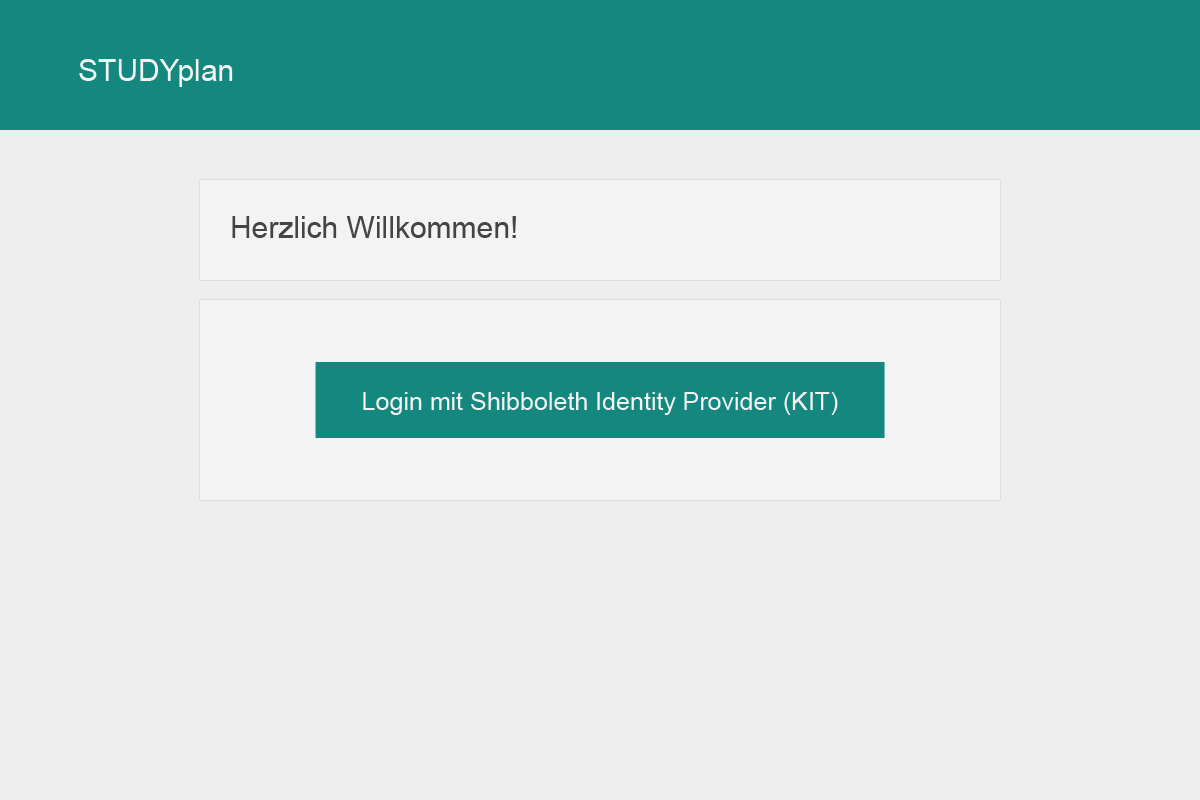
\includegraphics[width=0.8\textwidth]{../GUI/ergebnisse/login-1.png}
\end{figure}
\begin{figure}[!h]
	\caption{Erste Seite des Registrierungs"=\gls{Wizard}s mit Eingabe von Studienfach und Studienbeginn}
	\label{fig:gui-registrierung-1}
	\centering
	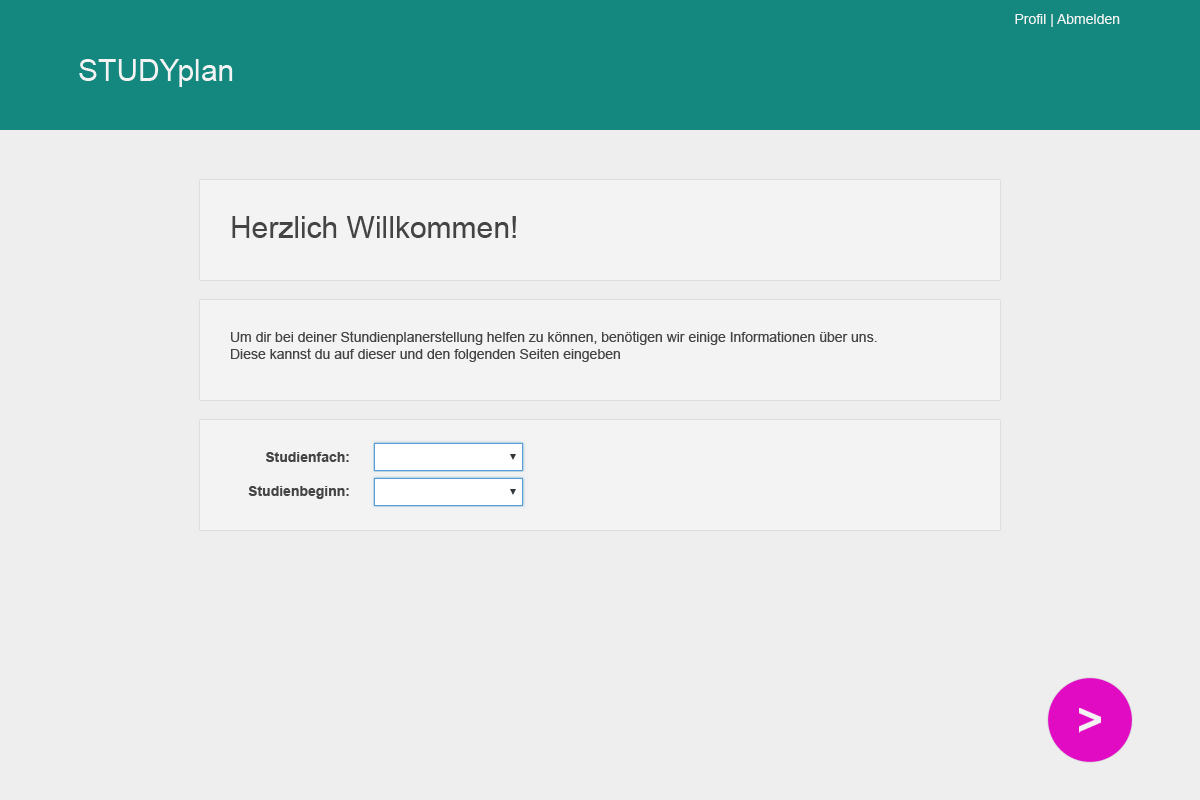
\includegraphics[width=0.8\textwidth]{../GUI/ergebnisse/registrierung-1.png}
\end{figure}

\begin{figure}
	\caption{Zweite Seite des Registrierungs"=\gls{Wizard}s mit Eingabe der schon begonnenen Module}
	\label{fig:gui-registrierung-2}
	\centering
	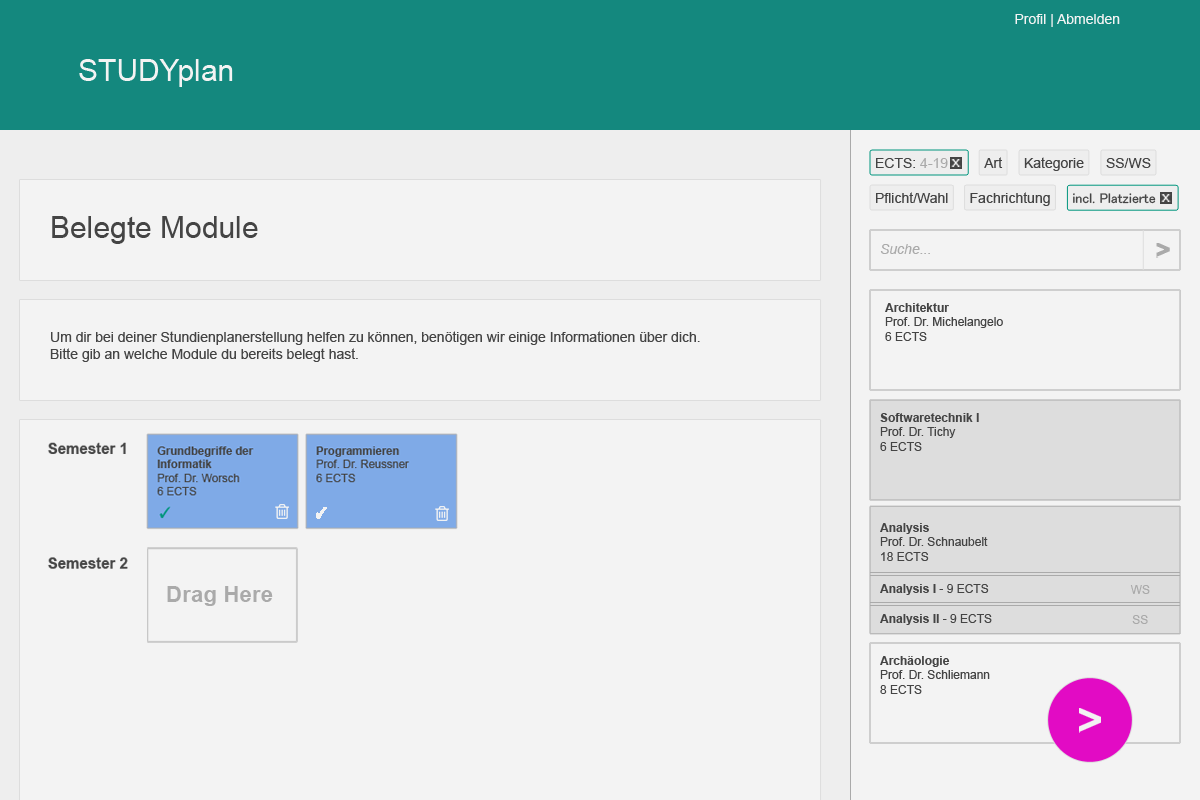
\includegraphics[width=0.9\textwidth]{../GUI/ergebnisse/registrierung-2.png}
\end{figure}

\begin{figure}
	\caption{Hauptseite des Systems}
	\label{fig:gui-hauptseite-1}
	\centering
	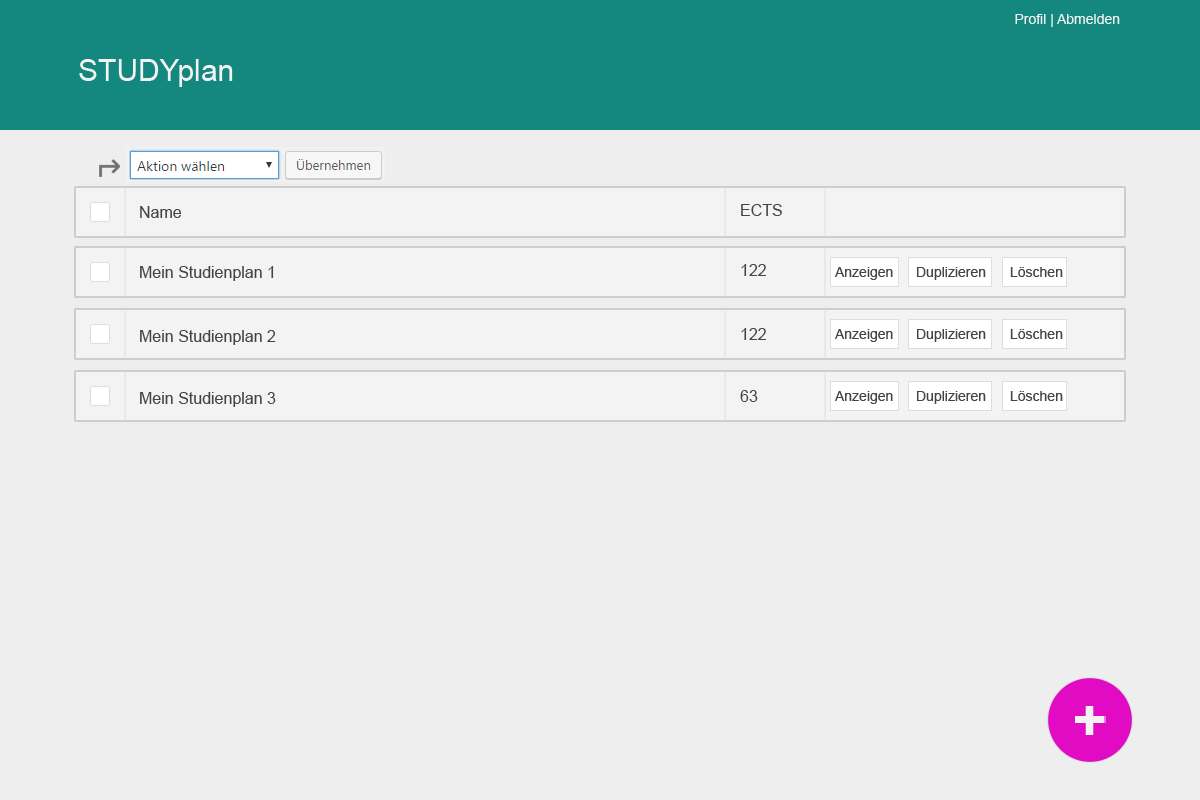
\includegraphics[width=0.9\textwidth]{../GUI/ergebnisse/hauptseite-1.png}
\end{figure}
\begin{figure}
	\caption{Manuelle Bearbeitung des Studienplans}
	\label{fig:gui-bearbeitung-1}
	\centering
	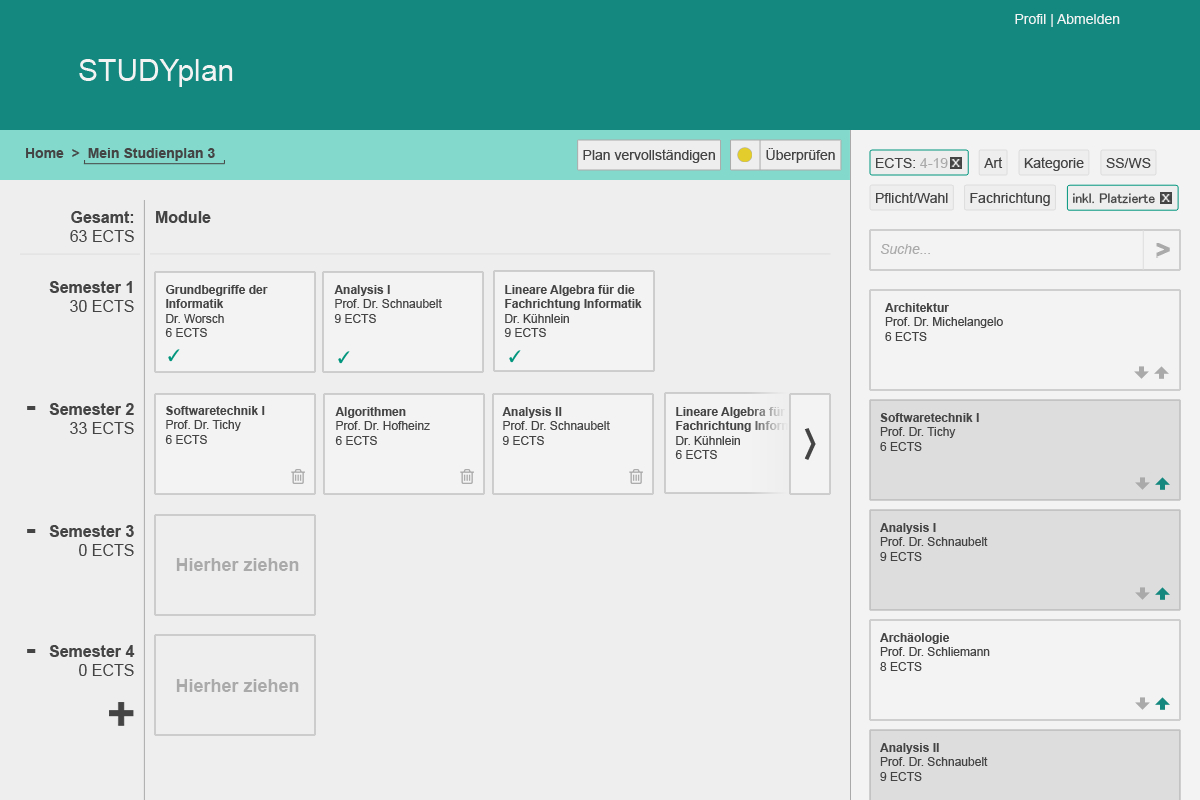
\includegraphics[width=0.9\textwidth]{../GUI/ergebnisse/bearbeitung-1.png}
\end{figure}
\begin{figure}
	\caption{Seitenleiste für Modulfilterung mit offener Kategorie-Auswahl}
	\label{fig:gui-module-filtern-1}
	\centering
	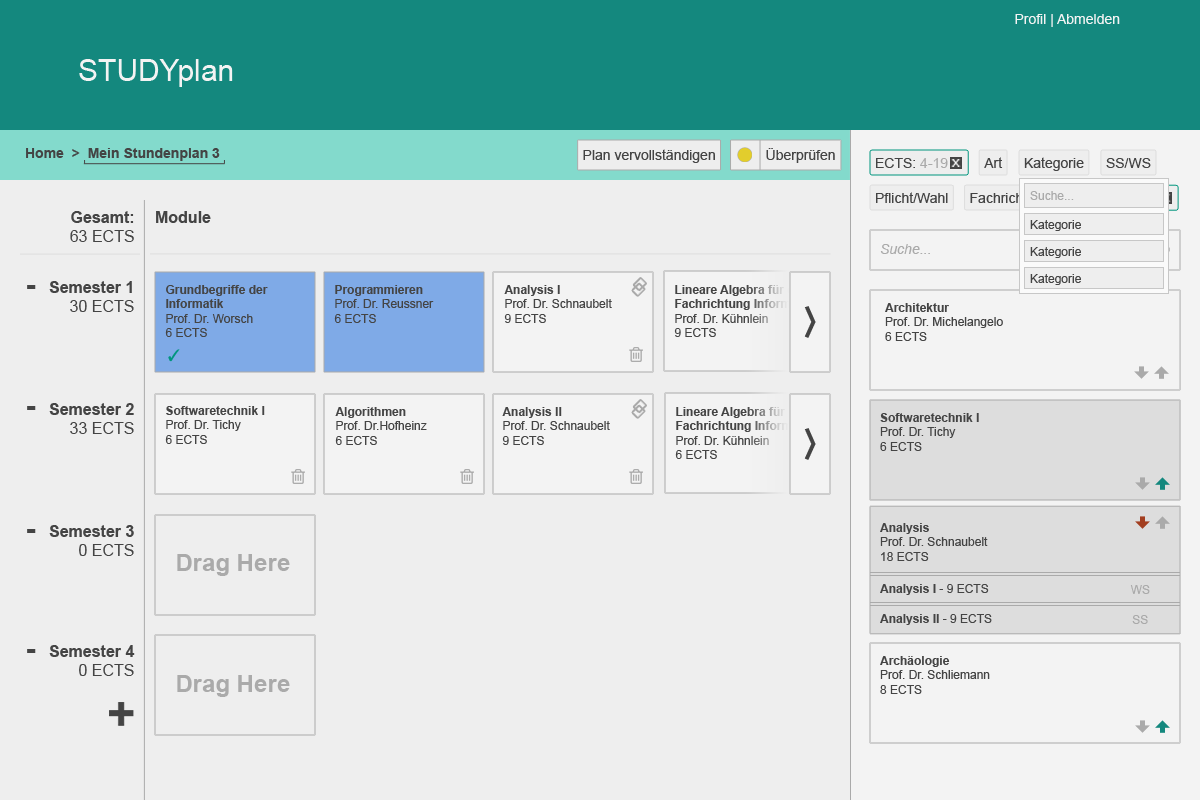
\includegraphics[width=0.9\textwidth]{../GUI/ergebnisse/module-filtern-1.png}
\end{figure}
\begin{figure}
	\caption{Seitenleiste für Modulfilterung mit offener ECTS-Auswahl}
	\label{fig:gui-module-filtern-2}
	\centering
	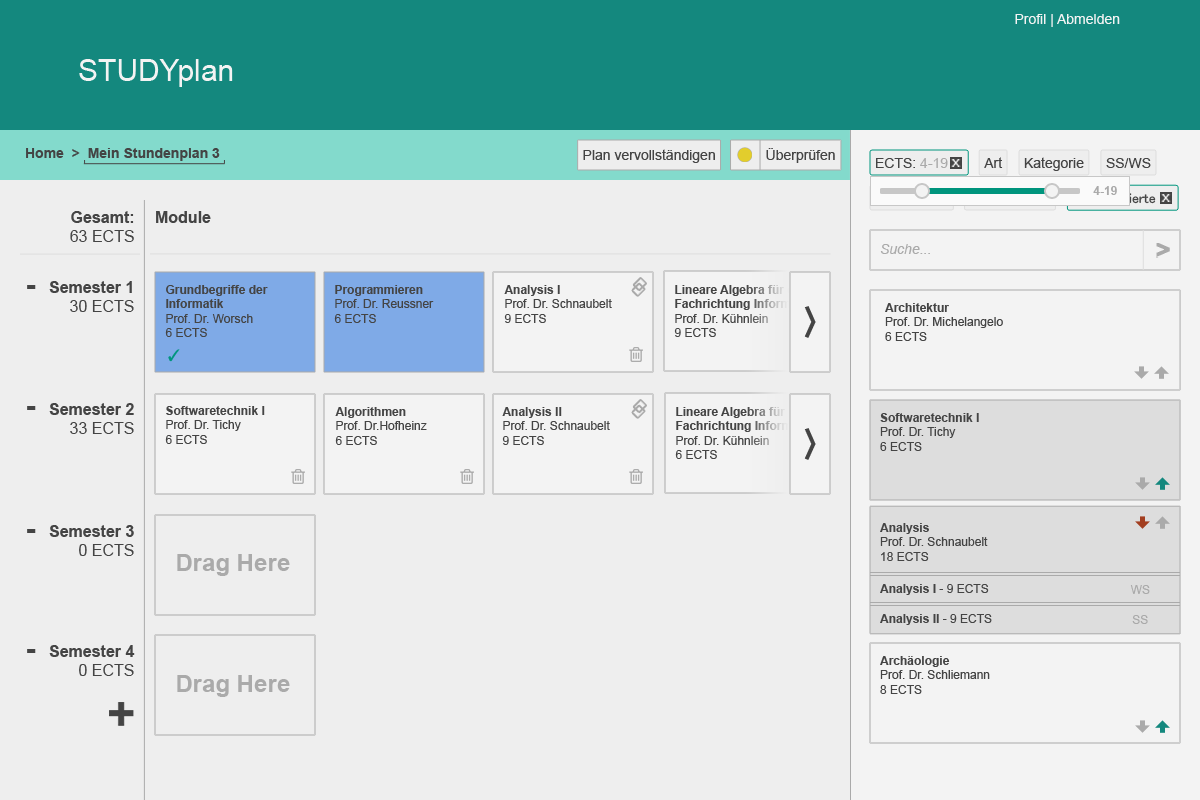
\includegraphics[width=0.9\textwidth]{../GUI/ergebnisse/module-filtern-2.png}
\end{figure}
\begin{figure}
	\caption{Detailansicht für Modul}
	\label{fig:gui-modul-info-1}
	\centering
	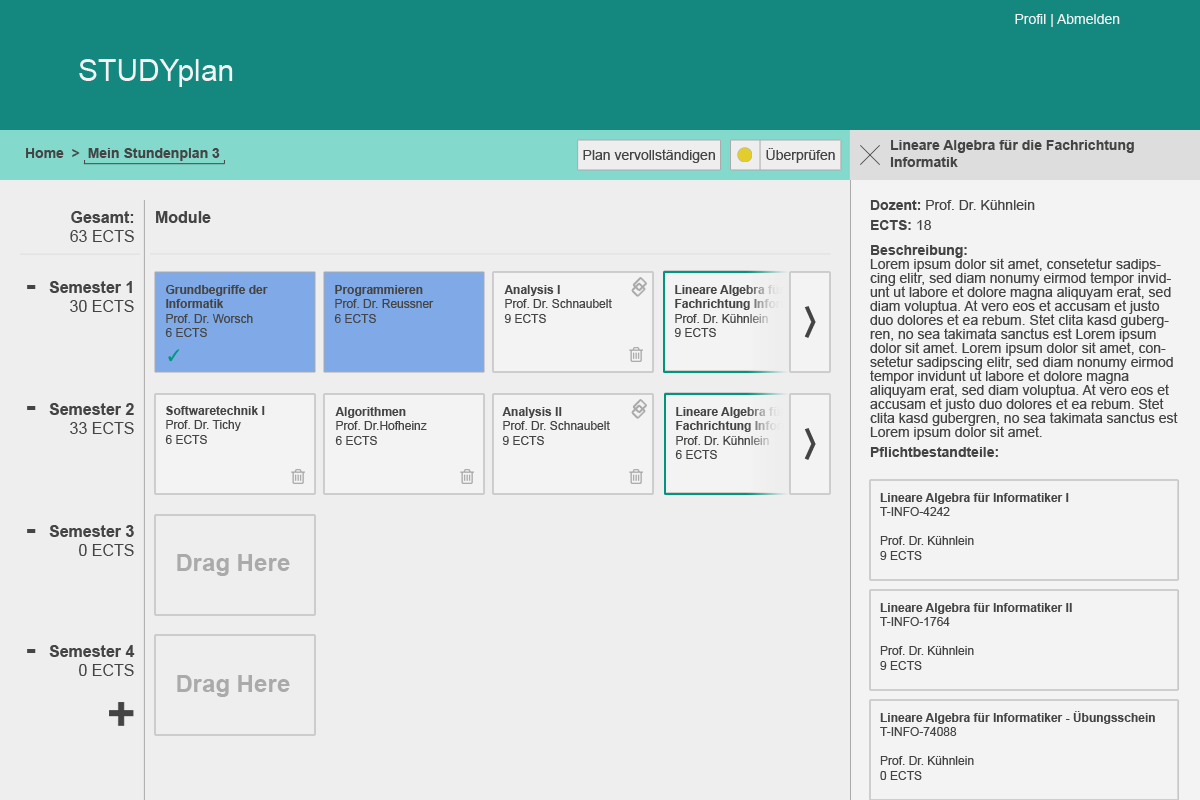
\includegraphics[width=0.9\textwidth]{../GUI/ergebnisse/modul-info-1.png}
\end{figure}
\begin{figure}
	\caption{1. Seite des Generierungs-Wizards}
	\label{fig:gui-generierung-1}
	\centering
	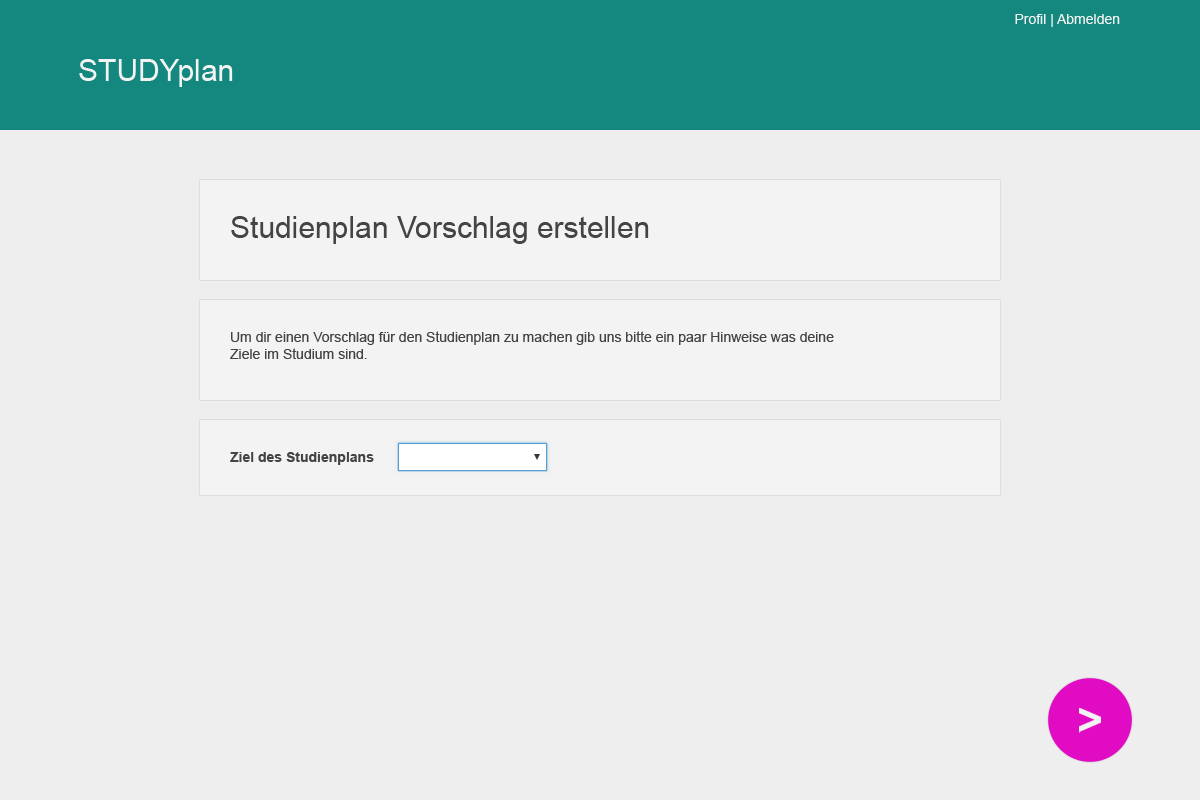
\includegraphics[width=0.9\textwidth]{../GUI/ergebnisse/generierung-1.png}
\end{figure}

\begin{figure}
	\caption{2. Seite des Generierungs-Wizard}
	\label{fig:gui-generierung-2}
	\centering
	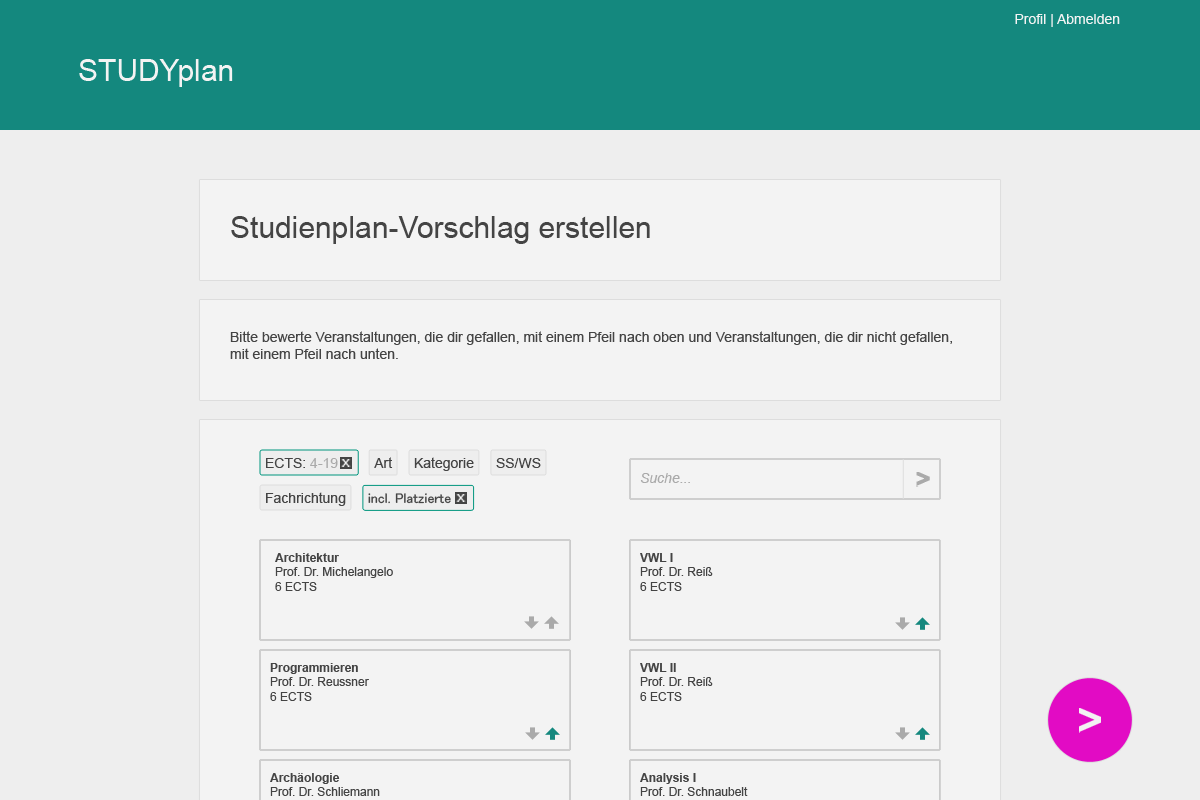
\includegraphics[width=0.9\textwidth]{../GUI/ergebnisse/generierung-2.png}
\end{figure}

\begin{figure}
	\caption{3. Seite des Generierungs-Wizard}
	\label{fig:gui-generierung-3}
	\centering
	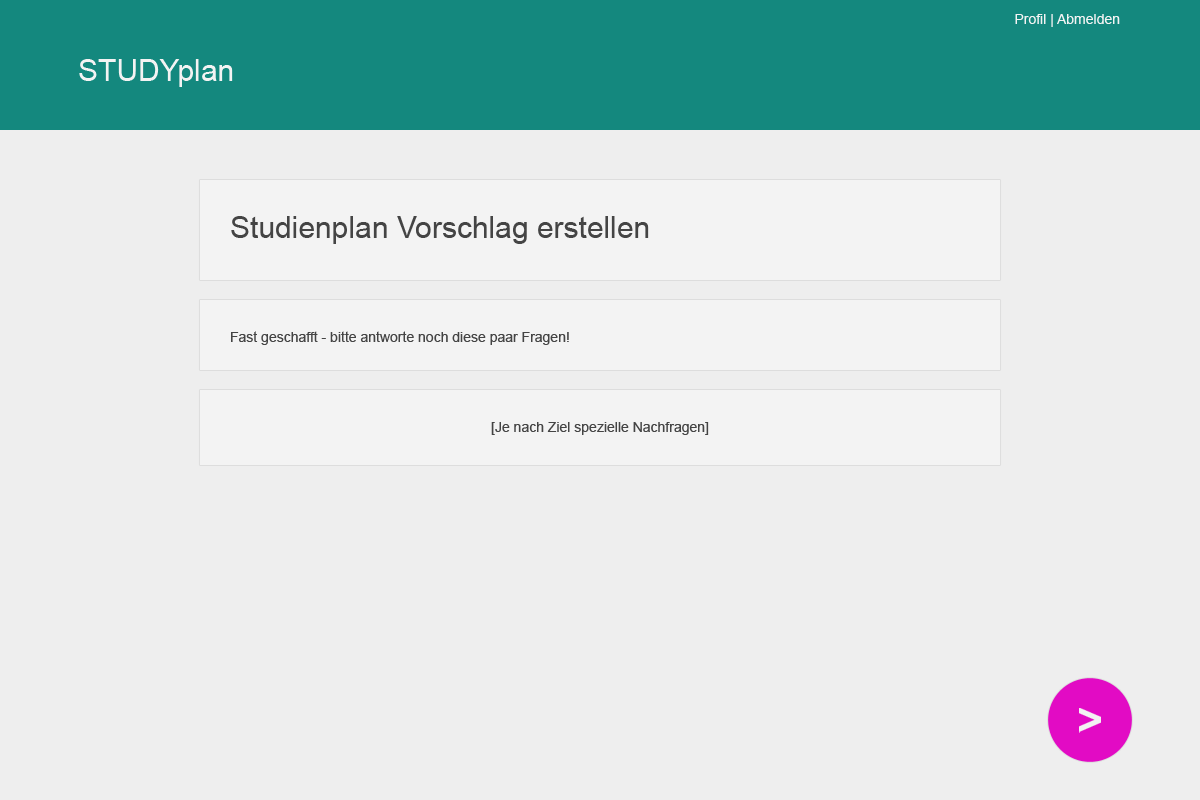
\includegraphics[width=0.9\textwidth]{../GUI/ergebnisse/generierung-3.png}
\end{figure}

\begin{figure}
	\caption{Anzeige des generierten Studienplans}
	\label{fig:gui-generierung-4}
	\centering
	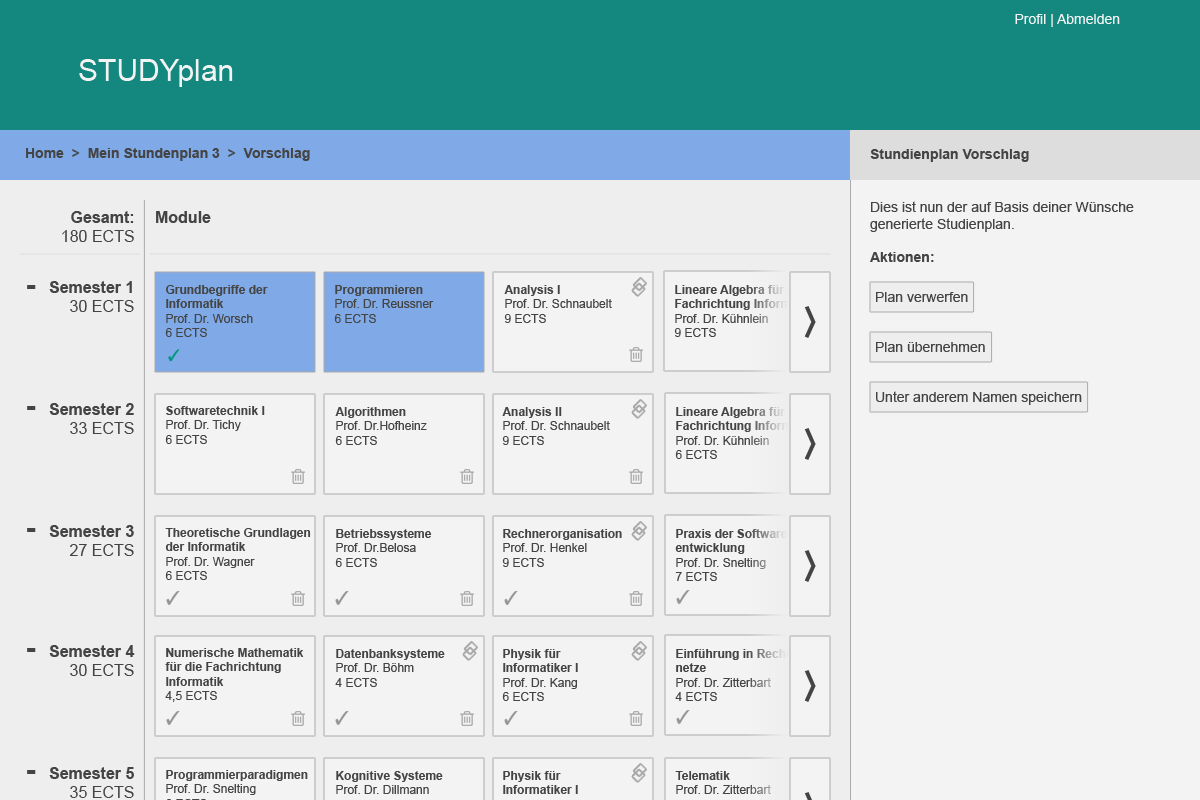
\includegraphics[width=0.9\textwidth]{../GUI/ergebnisse/generierung-4.png}
\end{figure}
\begin{figure}
	\caption{Erfolgreiche Verifizierung}
	\label{fig:gui-verifizierung-1}
	\centering
	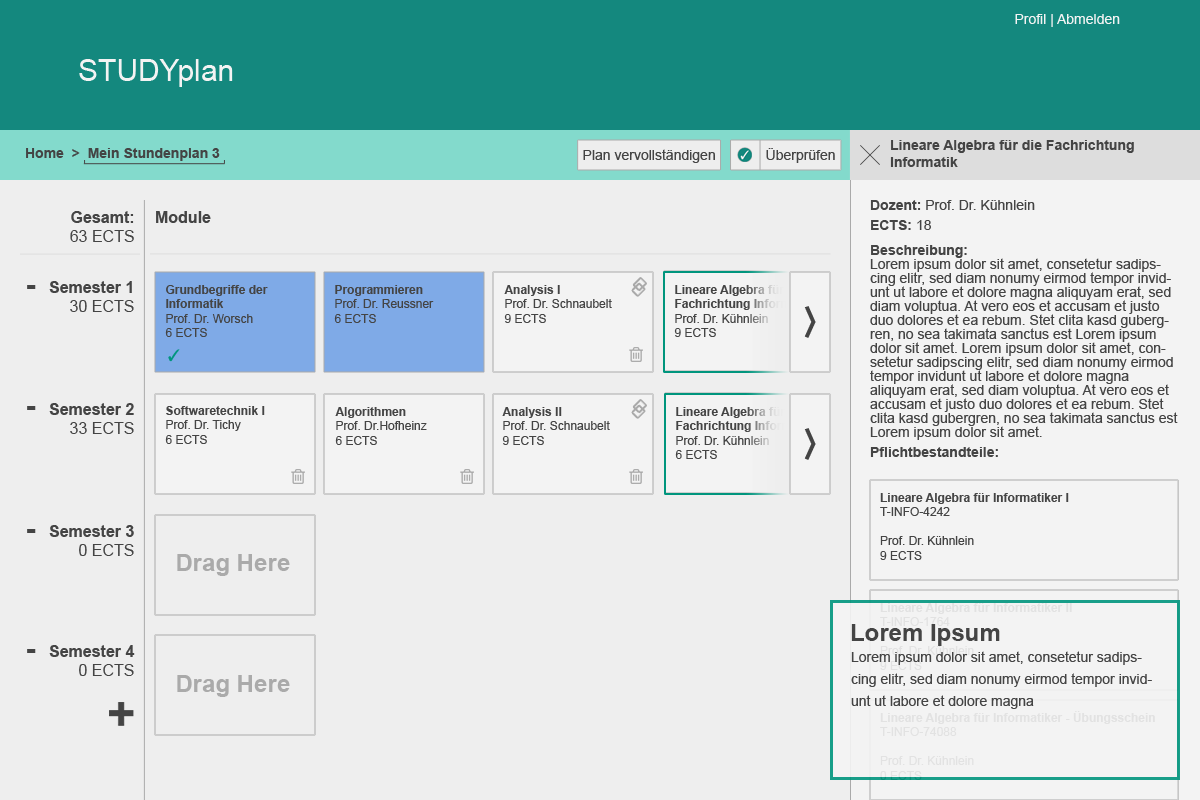
\includegraphics[width=0.9\textwidth]{../GUI/ergebnisse/verifizierung-1.png}
\end{figure}
\begin{figure}
	\caption{Fehlgeschlagene Verifizierung}
	\label{fig:gui-verifizierung-2}
	\centering
	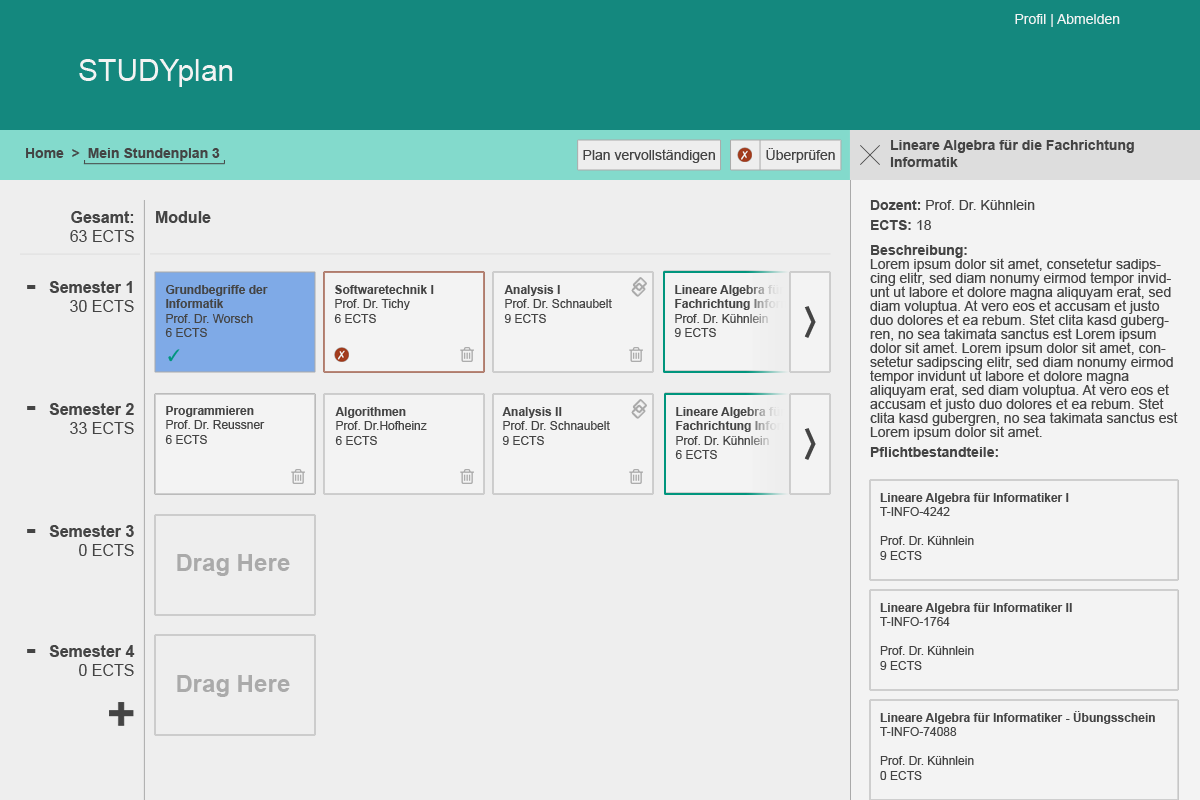
\includegraphics[width=0.9\textwidth]{../GUI/ergebnisse/verifizierung-2.png}
\end{figure}
\begin{figure}
	\caption{Profilansicht}
	\label{fig:gui-profil-1}
	\centering
	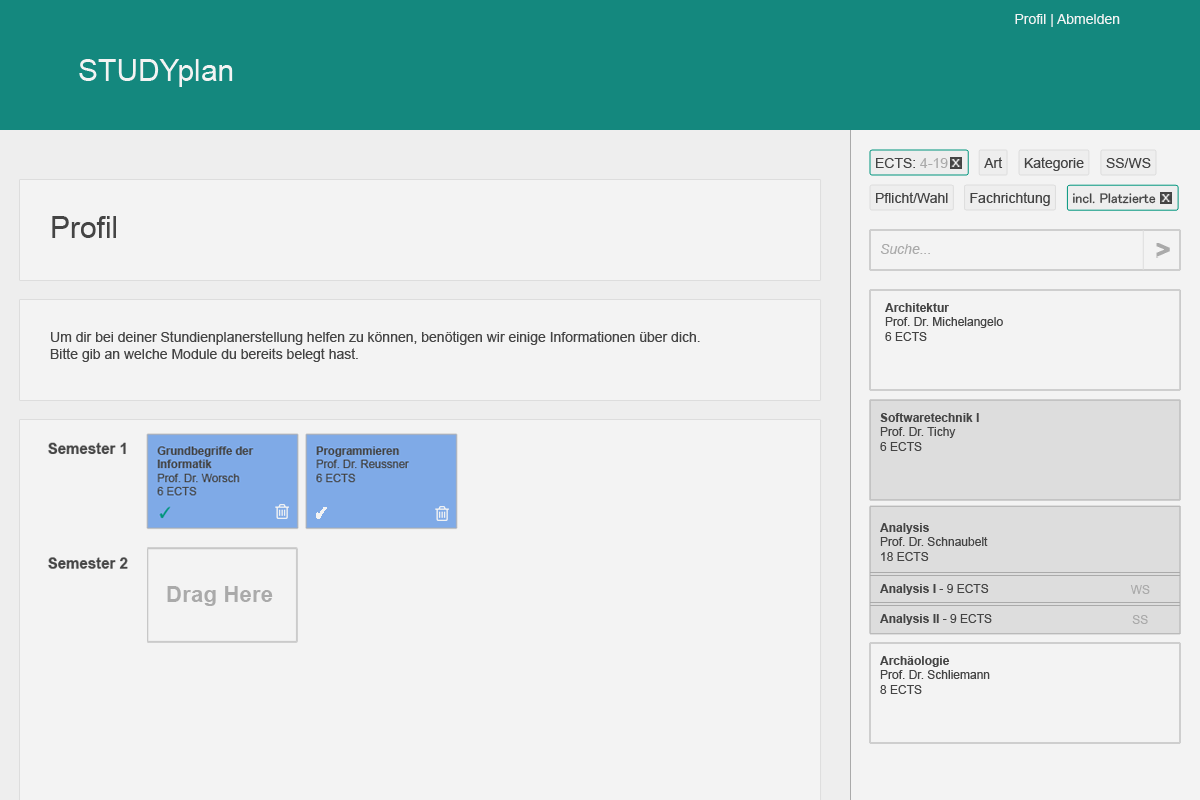
\includegraphics[width=0.9\textwidth]{../GUI/ergebnisse/profil-1.png}
\end{figure}
\FloatBarrier	
%\end{appendices}
\end{document}
